\chapter{Information Retrieval}
\label{chap:Information_Retrieval}

Information retrieval (IR) is an activity to extract information relevant to a
given information from a collection of information resources. The search can be based
on {\it metadata} or full-text (or other content-based) indexing. When the data
is huge, {\bf automated information retrieval} is important.

The idea of using computer to do IR started as early as 1945, from an article
``As We May Think'' by Vannevar Bush. The first automated IR was built in 1950s
and 1960s. Web-search engine is a form of very-large scale IR applications.

To do automated IR, the documents are often transformed or represented in some
form. This is called a model and is categorized according to 2 dimensions: {\it
mathematical basis} and the {\it properties of the model},
Fig.\ref{fig:IR_classification}.

\begin{figure}[hbt]
  \centerline{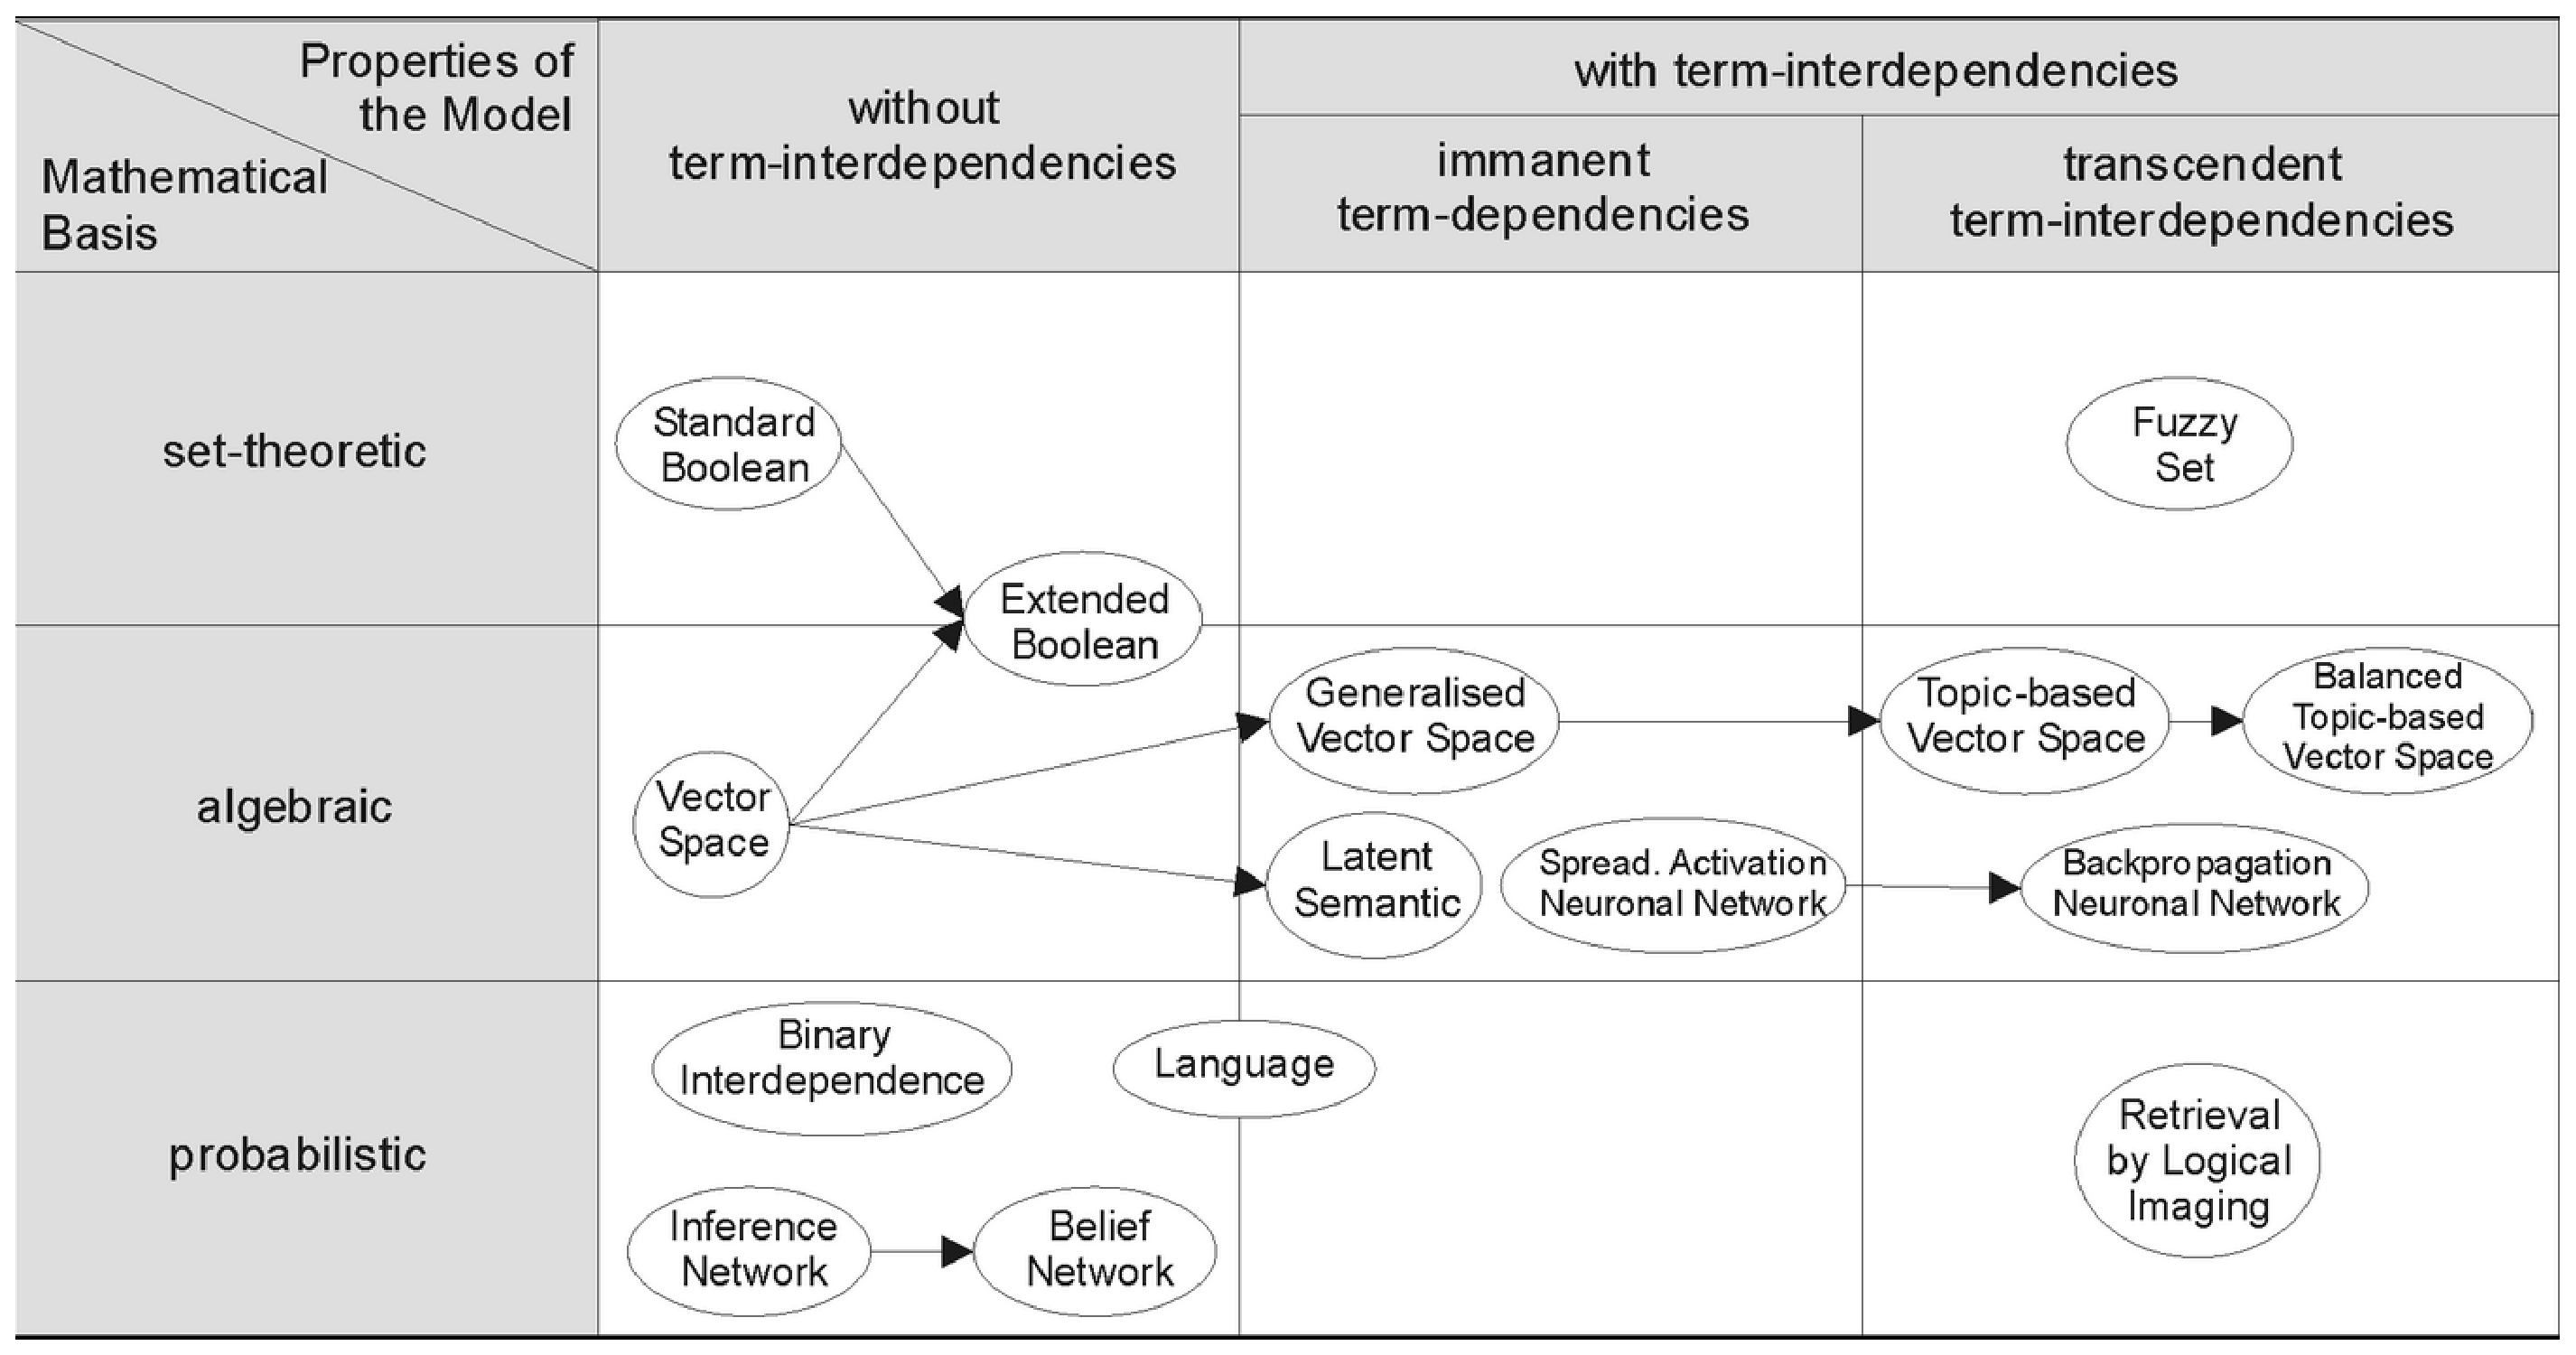
\includegraphics[height=5cm,
    angle=0]{./images/IR_classification.eps}}
\caption{Categorization of IR-models}
\label{fig:IR_classification}
\end{figure}


Libraries to do IR
\begin{enumerate}
  \item ElasticSearch (Chap.\ref{chap:elastic_search})
  \item Lemur 
  \item Lucene (Sect.\ref{sec:Lucene})
  \item Solr (Chap.\ref{chap:Solr})
  \item Sphinx
  \item Xapian
  \item Terrier Search Engine
\end{enumerate}
\url{http://en.wikipedia.org/wiki/List_of_information_retrieval_libraries}